\documentclass[12pt, a4paper]{report}

\usepackage[utf8x]{inputenc}
\usepackage{amsmath}
\usepackage[english,russian]{babel}
\usepackage{cmap}
\usepackage{listings}
\usepackage{geometry}
 \geometry{
 a4paper,
 total={170mm,257mm},
 left=20mm,
 top=20mm,
 }

 \def\Tp{0.0014}
 \def\Tk{0.23}
 \def\Kp1{4}
 \def\Td{2}
 \def\Kd1{1}

 \def\AAAA{0.0028}
 \def\AAA{0.4614}
 \def\AA{2.23}
 \def\A{5}

 \def\D{0.46}
 \def\DD{1.01}
 \def\DDD{5.07}

 \def\cc{13.58}
 \def\xx{5.41}

\usepackage{graphicx}
\graphicspath{ {../images/.} }

\begin{document}
\section*{Введение}
\textbf{Устойчивость} - свойство САР(системы автоматического регулирования) возвращаться к устойчивому установившемуся режиму после оказания внешнего воздействия. \\

\text{Различают 3 вида устойчивости:}
\begin{enumerate}
  \item[a.] Устойчивое
  \item[б.] Не устойчивое
  \item[в.] Граница устойчивости
\end{enumerate}
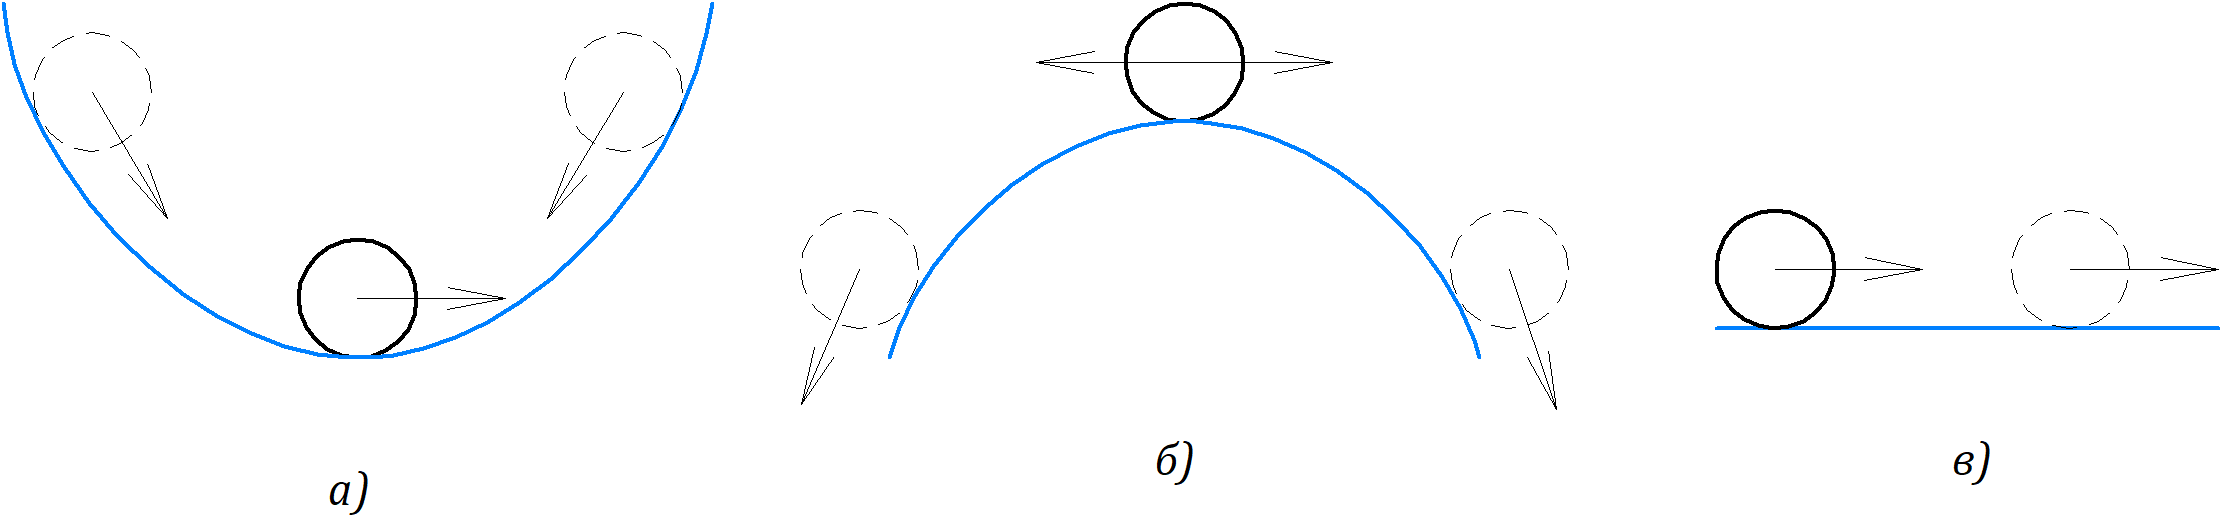
\includegraphics[width=15cm, height=4cm]{condition}

\textbf{Устойчивость САР оценивается по:}
\begin{enumerate}
  \item Статическим характеристикам
  \item По экспериментально полученным переходным процессам
  \item По математическому описанию
\end{enumerate}

\textbf{Условие устойчивости по математическому описанию САР}
\[ \lim\limits_{ t\rightarrow\infty}{\varphi_{пер}(t)} = 0\]
\[ \lim\limits_{ t\rightarrow\infty}{\omega(t)} = 0\]
\[ \varphi_{пер}(t) = C * e^{pt}, \]
\centerline{где p - корни характеристического уравнения.}\\

\centerline{\textbf{Характеристическое уравнение САР}}
\begin{displaymath}
a(p) = a_{0}p^n + a_{1}p^{n-1} + \ldots + a_{n-1}p + a_{n}
\end{displaymath}
В текущей работе будет рассмотрена система 3-го порядка $$ a(p) = A_{3}p^3 + A_{2}p^2 + A_{1}p + A_{0} $$
Параметры хар.уравнения
$$ A_{3} = Tp^2Td $$
$$ A_{2} = Tp^2 + TkTd $$
$$ A_{1} = Tk+Td $$
$$ A_{0} = 1 + Kp1Kd1 $$

\newpage
\textbf{Оценка устойчивости CАР по расположению корней характеристического уравнения.} \\
Для устойчивости САР необходимо и достаточно, чтобы все корни лежали в левой полуплоскости плоскости корней.
Условие выполняется если корни отрицательны или комплексно сопряженные с отрицательной вещественной частью
\begin{displaymath}
\varphi_{\text{пер}}(t) = C_{1}e^{p_{1}t} + C_{2}e^{p_{2}t} + C_{3}e^{p_{3}t} =
\frac{C_{1}}{e^{t}} + \frac{C_{2}}{e^{2t}} + \frac{C_{3}}{e^{3t}}
\end{displaymath}

Для систем высоких порядков нахождение корней становится трудоемким и желательно знать признаки устойчивости
САР без нахождения корней характеристического уравнения.\\

\textbf{Критерии устойчивости}
\begin{enumerate}
 \item Критерий устойчивости Рауcа-Гурвица
 \item Оценка устойчивости и характера переходного процесса\\по диаграмме Вышнеградского
 \item Критерий устойчивости Михайлова
 \item Следствие из критерия устойчивости Михайова
 \item Критерий устойчивости Найквиста
 \item Синтез САР по устойчивости по методу D-разбиения
\end{enumerate}

\textbf{Исходные данные}:
$$ Tp = \Tp $$
$$ Tk = \Tk $$
$$ Kp1 = \Kp1 $$
$$ Td = \Td $$
$$ Kd1 = \Kd1 $$
$$ \downarrow $$
$$ A_{3} = \AAAA \:c^{3} $$
$$ A_{2} = \AAA \:c^{2}$$
$$ A_{1} = \AA \:c$$
$$ A_{0} = \A $$

\newpage
1. Критерий устойчивости \textbf{Рауcа-Гурвица}.

Для устойчивости САР необходимо, чтобы все коэффициенты были положительны и достаточно, чтобы были положительны n определителей Гурвица
Необходимое условие
$$ A_{3} > 0, A_{2} > 0, A_{1} > 0, A_{0} > 0 $$

Матрица Гурвица
Пусть дан полином с вещественными коэффициентами: $$ a(p) = a_{0}p^n + a_{1}p^{n-1} + \ldots + a_{n-1}p + a_{n}$$

Тогда квадратичная матрица n * n

$$
    H = \begin{pmatrix}
        a_{1}  &a_{3}  &a_{5}  &\dots  &\dots  &\dots  &0      &0      &0\\
        a_{0}  &a_{2}  &a_{4}  &       &       &       &\vdots  &\vdots  &\vdots \\
        0      &a_{1}  &a_{3}  &       &       &       &\vdots  &\vdots  &\vdots \\
        0      &a_{0}  &a_{2}  &\ddots &       &       &0       &\vdots  &\vdots \\
        \vdots &0      &a_{1}  &       &\ddots &       &a_{n}   &0       &\vdots \\
        \vdots &0      &a_{0}  &       &       &\ddots &a_{n-1} &0       &\vdots \\
        \vdots &\vdots &0      &       &       &       &a_{n-2} &a_{n}   &0      \\
        \vdots &\vdots &\vdots &       &       &       &a_{n-3} &a_{n-1} &0      \\
        0      &0      &0      &\dots  &\dots  &\dots  &a_{n-4} &a_{n-2} &a_{n}  \\
        \end{pmatrix}
$$

Называется \textbf{матрицей Гурвица}, соответствующей полиному a(p)

Миноры
$$
    \Delta_{1}(p) = \begin{vmatrix}
                    a_{1}
                    \end{vmatrix}
$$

$$
   \Delta_{2}(p) = \begin{vmatrix}
                    a_{1} &a_{3} \\
                    a_{0} &a_{2}
                    \end{vmatrix}
$$

$$
   \Delta_{3}(p) = \begin{vmatrix}
                    a_{1} &a_{3} &a_{5}\\
                    a_{0} &a_{2} &a_{4}\\
                    0     &a_{1} &a_{3}
                    \end{vmatrix}
$$

вида $ {\textstyle \Delta _{k}(p)} $ называются \textbf{определителями Гурвица}. Для устойчивости САР достаточно, чтобы первые n определителей Гурвица были положительны
Для наших входных параметров имеем:
$$
    \Delta_{1}(p) = \begin{vmatrix}
                    \AAA
                    \end{vmatrix} = \D
$$

$$
   \Delta_{2}(p) = \begin{vmatrix}
                    \AAA &a\A \\
                    \AAAA &\AA
                    \end{vmatrix} = \DD
$$

$$
   \Delta_{3}(p) = \begin{vmatrix}
                    \AAA  &\A   &0\\
                    \AAAA &\AA  &0\\
                    0     &\AAA &\A
                    \end{vmatrix} = \DDD
$$

По критерию Рауса-Гурвица \textbf{САР устойчива}.


\newpage
2. Оценка устойчивости и характера переходного процесса по \textbf{диаграмме Вышнеградского}.

Для использования данного метода преобразуем выражение:
$$ A_{3}\frac{d^{3}\varphi}{dt^{3}} + A_{2}\frac{d^{2}\varphi}{dt^{2}} + A_{1}\frac{d\varphi}{dt} + A_{0}\varphi = 0 $$

1. Делим все слагаемые на A3:
$$ \frac{d^{3}\varphi}{dt^{3}} + \frac{A_{2}}{A_{3}}\frac{d^{2}\varphi}{dt^{2}} + \frac{A_{1}}{A_{3}}\frac{d\varphi}{dt} + \frac{A_{0}}{A_{3}}\varphi = 0 $$

2. Вводим новую переменную:
$$ t = q\tau $$ где t - время, q - масштабный коэффициент, $\tau$ - время
$$ \frac{d^{3}\varphi}{q^{3}d\tau^{3}} + \frac{A_{2}}{A_{3}}\frac{d^{2}\varphi}{q^{2}d\tau^{2}} + \frac{A_{1}}{A_{3}}\frac{d\varphi}{qdt} + \frac{A_{0}}{A_{3}}\varphi = 0 $$

3. Умножаем на $ q^3 $:
$$ \frac{d^{3}\varphi}{d\tau^{3}} + q\frac{A_{2}}{A_{3}}\frac{d^{2}\varphi}{d\tau^{2}} + q^{2}\frac{A_{1}}{A_{3}}\frac{d\varphi}{dt} + q^{3}\frac{A_{0}}{A_{3}}\varphi = 0 $$
При этом подбираем масштабный коэффициент q так, чтобы выполнялось равенство $$ \int{ \frac{A_{0}}{A_{3}}q^{3} } = 1 \Rightarrow q = \sqrt[3]{\frac{A_{3}}{A_{0}}} $$


4. Уравнение в нормированном виде:
$$ \frac{d^{3}\varphi}{d\tau^{3}} +
        \sqrt[3]{\frac{A_{3}}{A_{0}}}\frac{A_{2}}{A_{3}}\frac{d^{2}\varphi}{d\tau^{2}} +
        \sqrt[3]{\frac{A_{3}^{2}}{A_{0}^{2}}}\frac{A_{1}}{A_{3}}\frac{d\varphi}{dt} +
        \varphi = 0 $$

Критерии подобия переходного процесса: $$ \chi = \frac{A_{2}}{\sqrt[3]{A_{3}^2A_{0}}}, \xi = \frac{A_{1}}{\sqrt[3]{A_{3}A_{0}^2}} $$

Итоговое уравнение $$ p^{3} + \chi p^{2} + \xi p + 1 = 0 $$

Достаточное условие $$ \Delta_{2} = \begin{vmatrix}
                                         a1 &a3 \\
                                         a0 &a2
                                         \end{vmatrix} =
                                         \begin{vmatrix}
                                         \chi &1 \\
                                         1    &\xi
                                         \end{vmatrix} $$

$$ \text{САР устойчива: } \Delta_{2} > 0 $$
$$ \text{САР на границе устойчивости: } \Delta_{2} = 0 $$
$$ \text{САР не устойчива: } \Delta_{2} < 0 $$

\newpage

\textbf{Для наших данных получаем:}
$$ \chi = \xx $$
$$ \xi = \cc $$
\includegraphics{chapter2}

Так как мы находимся выше кривой $ \chi\xi = 1 $ \textbf{САР устойчива}.

\newpage
3. \textbf{Критерий Михайлова}.

Чтобы САР (замкнутая или разомкнутая) была устойчивой, необходимо и достаточно, чтобы годограф $a(i\omega)$
при изменении $\omega$ от 0 до $ \infty $ переходил поочередно из квадранта в квадрант против часовой стрелки,
совершив при этом поворот на угол $\frac{\pi}{2}\cdot$ n, где n- степень полинома $a(i\omega)$

Для этого в наше уравнение подставим $ p = i\omega$
$$ a(p) = A_{3}p^{3} + A_{2}p^{2} + A_{1}p + A_{0} $$
$$ a(i\omega) = -iA_{3}\omega^{3} - A_{2}\omega^{2} + iA_{1}\omega + A_{0} = 0 $$

Представим уравнение в виде:
$$ a(i\omega) = X(\omega) + iY(\omega) $$

Тогда получим:
$$ \begin{cases}
        X(\omega) = -A_{2}\omega^{2} + A_{0} \\
        Y(\omega) = -A_{3}\omega^{3} + A_{1}\omega
        \end{cases}
$$

\includegraphics{chapter31}\\
\includegraphics{chapter32}

Наш полином имеет 3 порядок, у которого годограф $a(i\omega)$ проходит через 3 квадранта и совершает поворот на $ \frac{3\pi}{2} $.\\
Соответственно по критерию Михайлова \textbf{САР устойчива}.

\newpage
4. Следствие из критерия Михайлова\\
Для систем высокого порядка построение кривой Михайлова становится очень трудоёмким.
Для устойчивой САР необходимо и достаточно, чтобы при изменении $ \omega = 0\dots\infty $ корни вещественной $ X(\omega) $
и мнимой $ Y(\omega) $ частей вектора $ a(i\omega) $ последовательно чередовались

Следовательно, должно выполнятся соотношение
$$ \omega_{x1} < \omega_{y1} < \omega_{x2} < \omega_{y2} < \dots $$

Для САР 3-го порядка:
$$ a(i\omega) = X(\omega) + iY(\omega) $$

$$ \begin{cases}
        X(\omega) = -A_{2}\omega^{2} + A_{0} \\
        Y(\omega) = -A_{3}\omega^{3} + A_{1}\omega
        \end{cases}
$$

Тогда получим:
$ \omega_{x1} = 0 $, $ \omega_{y1} = \sqrt[2]{\frac{A_{0}}{A_{2}}} $, $ \omega_{x2} = \sqrt[2]{\frac{A_{1}}{A_{3}}} $

\includegraphics{chapter4}

Корни системы вещественной и мнимой частей чередуются.\\
Соответственно по следствию из критерия Михайлова \textbf{САР устойчива}.

\newpage
5. Критерий устойчивости \textbf{Найквиста}.

Позволяет оценить устойчивость замкнутой САР по виду АФЧХ соответствующей ей разомкнутой САР.
Для устойчивости замкнутой САР необходимо и достаточно, чтобы при $ \omega=0\ldots\infty $ $ \psi_1 $ вектора $ a_{1}(i\omega) $ составлял $ \psi_{1} = l_{p} * \pi $ в положительном направлении(против часовой стрелки), где $ l_{p} $ число корней зарактеристического уравнения разомкнутой САР расположенной в правой полуплоскости на плоскости корней

$$ W_{замкн}(p) = \frac{K_{р1}K_{д1}}{\underbrace{A_{3}p^{3} + A_{2}p^{2} + A_{1}p + A_{0}}_{\text{Хар.многочлен замкнутой САР}}} $$

$$ W_{разомк}(p) = \frac{K_{р1}K_{д1}}{\underbrace{A_{3}p^{3} + A_{2}p^{2} + A_{1}p + 1}_{\text{Хар.многочлен разомкнутой САР}}} $$

Подставим в уравнение разомкнутой САР $ p = i\omega $, домножив на комплексно-сопряжённое
$$ W_{разомк}(i\omega) = \frac{K_{р1}K_{д1}}{-A_{3}\omega^{3} - A_{2}\omega^{2} + iA_{1}\omega + 1}*
    \frac{1-A_{2}\omega^{2}-i(A_{1}\omega-A_{3}\omega^{3})}{1-A_{2}\omega^{2}-i(A_{1}\omega-A_{3}\omega^{3})} $$

Получим
$$ W_{разомк}(i\omega) = \frac{K_{р1}K_{д1}*(1-A_{2}\omega^{2})} {\underbrace{(1-A_{2}\omega^{2})^{2}+(A_{1}\omega-A_{3}\omega^{3})^{2}}_{Uразомк(\omega)}} +
    i\frac{-K_{р1}K_{д1}*(A_{1}\omega-A_{3}\omega^{3})} {\underbrace{(1-A_{2}\omega^{2})^{2}+(A_{1}\omega-A_{3}\omega^{3})^{2}}_{Vразомк(\omega)}} $$

\includegraphics{chapter51}\\
\includegraphics{chapter52}

В нашем случае можем воспользоваться упрощенной формой для случая устойчивой \textbf{разомкнутой САР}. \\
Для устойчивости САР необходимо и достаточо, чтобы АФЧХ разомкнутой САР не охватывала точку (-1, 0).

В нашем случае АФЧХ не охватывает точку (-1, 0), соответственно \textbf{САР устойчива}.

\newpage
6. Синтез САР по устойчивости по методу \textbf{D-разбиения(1 параметр)}.

Данный метод отностистя к методам синтеза, которые нужны для опредления структуры или параметров САР из требований к системе.

Примем $ K_{p1} = \lambda$ как неизвестный параметр, необходимо найти диапазон значений, который обеспечит устойчивую работу нашей системы
Запишем развернутое характеристической уравнение
$$\underbrace{T_{p}^2T_{d}}_{A_{3}}p^{3} + \underbrace{(T_{p}^{2} + T_{k}T_{d})}_{A_{2}}p^{2} + \underbrace{(T_{k}T_{d})}_{A_{1}}p + 1 + K_{p1}K_{d1} = 0 $$

Подставив $ \lambda $ вместо $ K_{p1} $ получим
$$ T_{p}^2T_{d}p^{3} + (T_{p}^{2} + T_{k}T_{d})p^{2} + (T_{k}T_{d})p + 1 + \lambda K_{d1} = 0 $$

Выразим $ \lambda(p) $
$$ \lambda(p) = \frac{- A_{3}p^{3} - A_{2}p^{2} - A_{1}p - 1}{K_{d1}} $$

Подставим $ p = i\omega $ и преобразуем к виду $ \lambda(i\omega) = X(\omega) + iY(\omega) $
$$ \lambda(i\omega) = \frac{iA_{3}\omega^{3} + A_{2}\omega^{2} - iA_{1}p - 1}{K_{d1}} $$
$$ \begin{cases}
        X(\omega) = \frac{A_{2}\omega^{2} - 1}{K_{d1}} \\
        Y(\omega) = \frac{A_{3}\omega^{3} - A_{1}\omega}{K_{d1}}
        \end{cases}
$$

Правило штриховки на плоскости 1-го неизвестного параметра. При движении от точки $ \omega = -\infty $ к $ \omega = +\infty $
штриховка слева по ходу движения. Область вся заштрихованная изнутри является областью устойчивости.
Поскольку искомый параметр является вещественным числом, то из полученной области выделяются только точки, лежащие на вещественной оси.

\includegraphics[width=\textwidth, height=10cm]{chapter6}\\
Для исходный параметров, доступный диапазон имеет вид: -1.0 < Kp1 < 366.47

\end{document}